\documentclass[conference]{IEEEtran}
\usepackage[T1]{fontenc}
\usepackage[utf8]{inputenc}
\usepackage[spanish,es-noshorthands]{babel}
\usepackage{amsmath,amssymb,bm,graphicx,cite,booktabs,array,url}
\begin{document}
\title{Integración ROS 2--IRC5 y validación experimental de trayectorias LSPB en el ABB IRB 120}
\author{
\IEEEauthorblockN{Roberth Williams Ruiz Condori}
\IEEEauthorblockA{\textit{Ingeniería Mecatrónica}\\\textit{Universidad Católica Boliviana}\\Bolivia\\roberth.ruiz@ucb.edu.bo}
\and
\IEEEauthorblockN{Mario Alberto Nina Gallo}
\IEEEauthorblockA{\textit{Ingeniería Mecatrónica}\\\textit{Universidad Católica Boliviana}\\Bolivia\\mario.nina@ucb.edu.bo}}
\maketitle
\begin{abstract}
Se integró el modelo cinemático del ABB IRB 120 con ROS 2 Jazzy, RViz y el controlador IRC5 mediante Robot Web Services (RWS) y RAPID v2. Se realizó un ensayo físico repetitivo de un triángulo de 100\,mm por lado, con tres ciclos y 21 destinos verificados. La duración LSPB de referencia fue 34.71\,s y la observada 45.83\,s. El RMSE articular de seguimiento fue 2.042$^\circ$, mientras que el mayor error final de llegada fue 0.01562$^\circ$. La reconstrucción cartesiana mediante FK de las mediciones articulares permitió contrastar la forma del recorrido con la referencia geométrica. Se distingue la planificación del computador de la interpolación interna de ABB.
\end{abstract}
\begin{IEEEkeywords}
ABB IRB 120, ROS 2, IRC5, RWS, RAPID, LSPB, seguimiento articular.
\end{IEEEkeywords}
\section{Introducción}
El Hito 2 desarrolló la cinemática directa e inversa, el Jacobiano y la planificación LSPB. El presente trabajo integra dichos modelos con el manipulador físico para el ECI-3/4 de IMT-342, con énfasis en la comunicación bidireccional y la trazabilidad del movimiento \cite{s12,s14}. El ensayo se limita al backend RAPID v2 original.
\section{Metodología}
\subsection{Integración cinemática y comunicación}
La aplicación se ejecuta en Fedora mediante Podman y ROS 2 Jazzy. RViz permite seleccionar y previsualizar movimientos. El coordinador transmite por Ethernet las consignas articulares al IRC5 mediante RWS y recibe sus estados y posiciones articulares. El modelo URDF visualiza la postura reportada por el controlador.

Se reutiliza la convención D--H estándar del Hito 2 para el IRB 120 de seis juntas revolutas \cite{abb}. La pose de la brida se obtiene mediante
\begin{equation}
{}^{0}\!T_6(\bm q)=\prod_{i=1}^{6}{}^{i-1}\!T_i(q_i).
\end{equation}
Los objetivos cartesianos se resuelven por Pieper, con filtrado de límites, continuidad de rama y validación FK. La planificación comprueba las envolventes de colisión frente a los cuatro muros nominales de la celda. La brida es la referencia del ensayo.
\subsection{Planificación LSPB y RAPID v2}
Cada tramo se planifica con un perfil articular sincronizado, con reposo en los extremos. Para desplazamiento $\Delta q_i$, duración $T$ y tiempo de mezcla $t_c$,
\begin{equation}
|\Delta q_i|=a_i t_c(T-t_c).
\end{equation}
Se emplearon límites de referencia de 0.6\,rad/s y 1\,rad/s$^2$. RAPID v2 ejecuta destinos mediante \texttt{MoveAbsJ}, con tiempo solicitado \texttt{\textbackslash T}, zona \texttt{fine} y \texttt{tool0}. El IRC5 realiza la interpolación interna. El cliente verifica el acuse terminal RAPID y la llegada dentro de $\pm0.30^\circ$ por eje. El LSPB es una referencia del host, no una consigna directa al servo.
\subsection{Protocolo experimental}
Se programó un triángulo equilátero horizontal de 100\,mm de lado, a 450\,mm de altura respecto a la base. Los vértices nominales, en milímetros, son
\begin{align*}
 A&=(258,-28.868,450),\\
 B&=(358,-28.868,450),\\
 C&=(308,57.735,450).
\end{align*}
Cada ciclo comprende siete destinos: aproximación, A, B, C, cierre en A, retirada y retorno a la postura inicial medida (HOME). Se realizaron tres ciclos con un destino por vértice. No se exige interpolación lineal exacta de ABB entre vértices.
\section{Resultados}
\begin{table}[!t]
\caption{Ensayo físico del 24/11/2026 (\texttt{f71aa1fa})}
\label{tab:lote}
\centering\footnotesize
\begin{tabular}{lr}
\toprule
Magnitud & Resultado \\
\midrule
Ciclos / destinos verificados & 3/3; 21/21 \\
Duración de referencia & 34.71\,s \\
Duración observada & 45.83\,s \\
Incremento temporal & 32.03\% \\
RMSE de seguimiento del lote & 2.042$^\circ$ \\
Error máximo de seguimiento & 18.363$^\circ$ \\
Mayor error final de llegada & 0.01562$^\circ$ \\
Muestras de seguimiento & 239 \\
Desviación cartesiana del plan & 4.89\,mm \\
Desviación FK--lado ideal (máx.) & 4.85\,mm \\
\bottomrule
\end{tabular}
\end{table}
El lote completó los 21 destinos con retorno a HOME y estado de verificación satisfactorio (Tabla~\ref{tab:lote}). La diferencia de 11.12\,s entre la duración observada y la referencia incluye la ejecución del controlador y los intervalos de comunicación y verificación de cada destino. No se atribuye íntegramente a una sola causa.
\begin{figure}[!t]
\centering
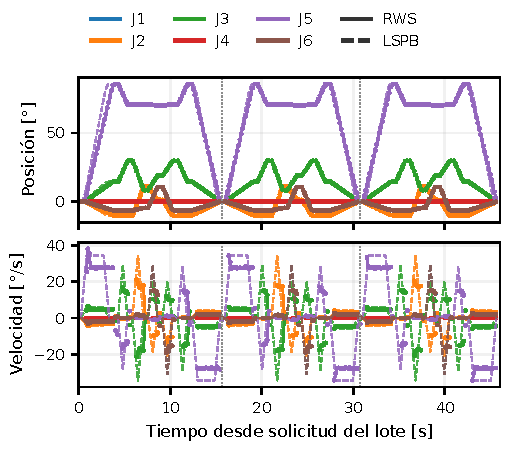
\includegraphics[width=\columnwidth]{figuras/seguimiento.pdf}
\caption{Posición y velocidad de las seis juntas en tres ciclos. Líneas continuas: posiciones RWS y velocidades estimadas a partir de las muestras; discontinuas: LSPB del host, alineado por tramo al inicio de fase 2 observado. Las líneas verticales punteadas delimitan ciclos.}
\label{fig:seguimiento}
\end{figure}
\subsection{Seguimiento articular}
La Fig.~\ref{fig:seguimiento} muestra el patrón repetitivo de las seis juntas. Se utilizaron 239 muestras RWS únicas en fase 2 dentro del intervalo de referencia, sin ajuste temporal, para las métricas registradas por la aplicación. El error de seguimiento se define como $e_i=q_i^{\mathrm{med}}-q_i^{\mathrm{ref}}$, con
\begin{equation}
\mathrm{RMSE}=\sqrt{\frac{1}{6N}\sum_{k=1}^{N}\sum_{i=1}^{6}e_i(k)^2}.
\end{equation}
El error transitorio máximo no equivale al error final: los 21 acuses terminales registraron errores finales inferiores a 0.016$^\circ$, dentro de la banda definida. La velocidad se estima mediante un ajuste cuadrático local de hasta cinco muestras RWS; no es una medición directa del servo. El intervalo mediano de recepción fue 0.152\,s para las 273 muestras únicas del lote retenidas para las gráficas.
\subsection{Reconstrucción cartesiana}
\begin{figure}[!t]
\centering
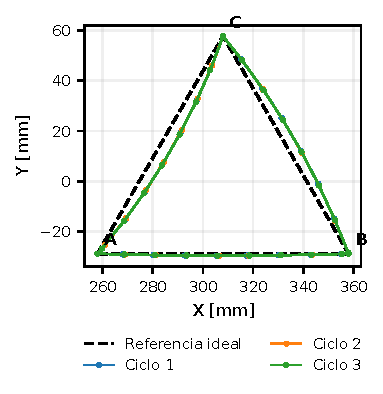
\includegraphics[width=0.92\columnwidth]{figuras/triangulo_xy.pdf}
\caption{Proyección XY de la brida reconstruida por FK a partir de RWS durante los tres trazados A--B--C--A. Se omiten la aproximación y la retirada.}
\label{fig:xy}
\end{figure}
La Fig.~\ref{fig:xy} compara los tres trazados con el triángulo ideal. Sobre 84 muestras de los lados, la distancia tridimensional al segmento ideal correspondiente presentó un RMS de 2.99\,mm y máximo de 4.85\,mm; el desvío vertical máximo muestreado fue 4.58\,mm. La desviación nominal de 4.89\,mm del plan es una magnitud distinta. La reconstrucción utiliza FK del modelo y no una medición cartesiana independiente.
\section{Discusión y conclusiones}
El sistema integró la cinemática, la generación de referencias, la ejecución temporizada y la realimentación articular del ABB IRB 120. Los tres ciclos muestran un patrón repetitivo, con todos los destinos verificados y un error final inferior a la tolerancia. La diferencia temporal y el error transitorio reflejan la distinción entre el perfil LSPB y la interpolación del IRC5. La forma reconstruida muestra un recorrido triangular con desviación de pocos milímetros en las muestras disponibles. El Jacobiano permite además identificar configuraciones cercanas a singularidad, especialmente al retornar a HOME. Los resultados caracterizan este ensayo y no constituyen una certificación metrológica de la precisión del robot.
\begin{thebibliography}{00}
\bibitem{s12} IMT-342 Robótica, ``Lanzamiento ECI-3/4 (Hito 3)'', Universidad Católica Boliviana, material docente, 2026; compilación \textit{S12\_material\_oficial.pdf}, pp. 7, 30.
\bibitem{s14} IMT-342 Robótica, ``Criterios unificados de validación cinemática, procedencia e incertidumbre (Hito 3)'', material docente, 2026; compilación \textit{S14\_material\_oficial.pdf}, pp. 4, 8. Propuesta sujeta a aprobación docente.
\bibitem{abb} ABB, \textit{IRB 120: Especificaciones del producto}, documento 3HAC035960-005, rev. W.
\end{thebibliography}
\end{document}
